\section{Introduction}
\label{sec:intro}

  Finite state automata are all-pervasive, adopting different roles in different contexts. We focus on the role of automata as \emph{formal models of system requirements} and their subsequent application in Model Based Testing (MBT). MBT is a paradigm in formal methods where the requirements of a system under test (SUT) are first converted to a formal model. This formal model is then used to automatically generate test cases for the SUT. There are many MBT tools (see \cite{10.1145/1353673.1353681,10.1002/stvr.456} for a survey) and in several of them, the formal model is given by some extension of finite automata. 

  Converting requirements to a Deterministic Finite Automaton (DFA) or a Non-deterministic Finite Automaton (NFA) is often cumbersome. This is because DFAs and NFAs describe low level computations which reason about individual actions. There are various ways in which automata can be made consise. In Generalized Automata~\cite{DBLP:books/lib/Eilenberg76,GIAMMARRESI1999191}, transitions contain words instead of single actions. A transition $q \xra{abb} q'$ is fired from $q$ if the word $abb$ is seen after the automaton reaches $q$. Therefore, requirements which depend on an exact sequence of actions can be represented using generalized automata more concisely. A natural extension is to allow for regular expressions in transitions, resulting in the model of Expression Automata~\cite{10.1007/978-3-540-30500-2_15} and its deterministic variant. Deterministic Expression Automata (DEA) impose restrictions on the regular expressions that can be used: they should result in a prefix-free language, and moreover, every pair of regular expressions out of state is language disjoint. This results in DEA recognizing a subset of regular languages. On the other hand, in (non-deterministic) Expression Automata, the transitions are so powerful that the states have almost no meaning: the entire automaton can be reduced to a single state and a single transition labeled by the regular expression representing the language. For languages leading to big automata, the corresponding regular expression can be complicated and incomprehensible. The goal is to hit a sweet spot where the transition labels are not too complicated, and at the same time there are fewer states than a DFA. 

   

  Deterministic suffix-reading automata (DSAs)~\cite{DBLP:journals/corr/abs-2410-22761} are a recently introduced automaton model for regular languages. Transitions are  labeled with words (as in a generalized automaton), however, the semantics is different. A transition $(q, abb, q')$ is fired from $q$ if a word \emph{ending} with the suffix $abb$ is seen. When there are multiple transitions out of a state, the first transition that matches is fired. Figure~\ref{fig:dsa-examples} gives some examples of DSAs.

  \begin{figure}
  \centering
  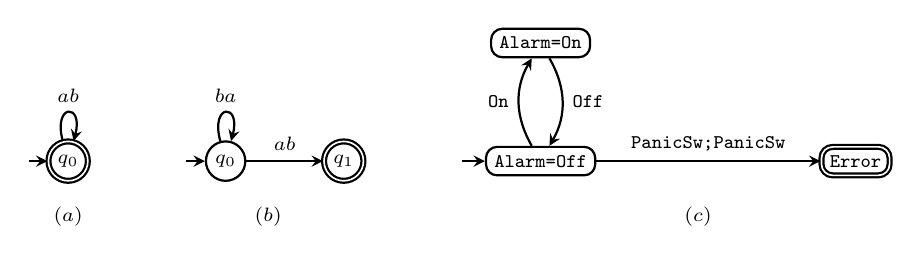
\begin{tikzpicture}[state/.style={circle, inner sep=2pt, draw, thick}]
    \begin{scope}[every node/.style={state}]
      \node [double] (0) at (0,0) {\scriptsize $q_0$};
    \end{scope}
    \begin{scope}[->, >=stealth, thick]
      \draw (-0.5, 0) to (0);
      \draw (0) to [loop above] node {\scriptsize $ab$} (0);
    \end{scope}
    \node at (0, -0.7) {\scriptsize $(a)$};

    \begin{scope}[xshift=2cm]
      \begin{scope}[every node/.style={state}]
        \node (0) at (0,0) {\scriptsize $q_0$};
        \node [double] (1) at (1.5, 0) {\scriptsize $q_1$};
      \end{scope}
      \begin{scope}[->, >=stealth, thick]
        \draw (-0.5, 0) to (0);
        \draw (0) to [loop above] node  {\scriptsize $ba$} (0);
        \draw (0) to node [above] {\scriptsize $ab$} (1);
      \end{scope}
      \node at (0.54, -0.7) {\scriptsize $(b)$};
    \end{scope}

      \begin{scope}[xshift=6cm]
        \begin{scope}
          \node [rectangle, rounded corners, draw, inner sep=3pt, thick] (0) at (0,0) {\scriptsize \texttt{Alarm=Off}};
          \node [rectangle, rounded corners, draw, inner sep=3pt, thick] (1) at (0,1.5) {\scriptsize \texttt{Alarm=On}};
          \node [rectangle, rounded corners, draw, inner sep=3pt, thick, double] (2) at (4, 0) {\scriptsize \texttt{Error}};
        \end{scope}

        \begin{scope}[->, >=stealth, thick]
          \draw (-1,0) to (0);
          \draw (0) to [bend left] node [left] {\scriptsize \texttt{On}} (1);
          \draw (1) to [bend left] node [right] {\scriptsize \texttt{Off}} (0);
          \draw (0) to node [above] {\scriptsize \texttt{PanicSw;PanicSw}} (2);
        \end{scope}
        \node at (2, -0.7) {\scriptsize $(c)$};
      \end{scope}
    
  \end{tikzpicture}
  \caption{Examples of Deterministic Suffix-reading Automata (DSA)}
  \label{fig:dsa-examples}
  \end{figure}

  In Figure~\ref{fig:dsa-examples}(a), the DSA accepts all words that end with $ab$, for instance $bab, bbab, babaab$, etc. The transition $q_0 \xra{ab} q_0$ is fired as soon as a word ending with $ab$ is seen after reaching $q_0$. For instance, on the word $babaab$, the transition is first triggered on the prefix $bab$ since this is the first time $ab$ appears as suffix; once the transition is triggered, the prefix $bab$ has been consumed, and now we are left with $aab$; on reading $aab$ fully, the transition $q_0 \xra{ab} q_0$ is triggered again.  In Figure~\ref{fig:dsa-examples}(b), we can view the state $q_0$ as tracking two suffixes $ba$ and $ab$. When $ba$ is seen before $ab$, the self-loop is triggered; otherwise when $ab$ is seen first, the transition to $q_1$ is taken. For example, on word $bbab$, the automaton starts at $q_0$, and on $bba$ it fires $q_0 \xra{ba} q_0$ (since $ba$ is a suffix of $bba$), then reads $b$ and remains there. %Since $q_0$ is non-accepting, the word is rejected. 
  However, on $bbaab$, the run loops on $bba$ back to $q_0$, and then reads the next $ab$ to reach $q_1$, and accept. The final example Figure~\ref{fig:dsa-examples}(c) is a \emph{suffix-based specification} of a part of an automotive software: when the alarm is off, and the panic switch is pressed twice within one second, flag an error. Here, we assume there is a symbol \texttt{tick} to denote the elapse of $1$ unit of time. So, on a word \texttt{tick}; \texttt{On}; \texttt{tick}; \texttt{Off}; \texttt{PanicSw}; \texttt{PanicSw}, an error should be flagged (we have added a separator symbol ; just for clarity). This specification is succinctly represented by the DSA in Figure~\ref{fig:dsa-examples}(c).

   Since transitions in a DSA wait for specific patterns to appear, DSAs are able to represent suffix-based specifications succinctly. When we consider systems with multiple components (which we call ports), the requirements can talk about different combinations of inputs. Here are two examples. 

   \begin{figure}
   \centering
   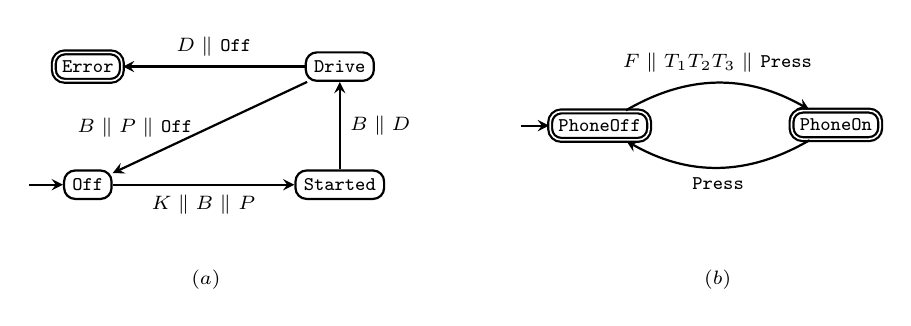
\begin{tikzpicture}
      \begin{scope}[every node/.style={rectangle, rounded corners, draw, inner sep=3pt, thick}]
        \node (0) at (0,0) {\scriptsize \texttt{Off}};
        \node [double] (1) at (0,1.5) {\scriptsize \texttt{Error}};
        \node (2) at (3.2,0) {\scriptsize \texttt{Started}};
        \node (3) at (3.2,1.5) {\scriptsize \texttt{Drive}};
      
      \end{scope}

      \begin{scope}[->,>=stealth, thick, auto]
        \draw (-0.75,0) to (0);
        %\draw (0) to [bend left] node [left] {\scriptsize \texttt{On}} (1);
        %\draw (1) to [bend left] node [right] {\scriptsize \texttt{Off}} (0);
        \draw (0) to node [below] {\scriptsize $K \parallel B \parallel$ $P$} (2);
        \draw (2) to node [right] {\scriptsize $B \parallel D$ } (3);
        \draw (3) to node [left] {\scriptsize $B \parallel P \parallel$ \texttt{Off}$~$} (0); 
        \draw (3) to node [above] {\scriptsize $D \parallel$ \texttt{Off}} (1);
      \end{scope}

      \node at (1.5, -1.2) {\scriptsize $(a)$};

      \begin{scope}[xshift=6.5cm]
        \begin{scope}[every node/.style={rectangle, rounded corners, draw, inner sep=3pt, thick}]
          \node [double] (0) at (0,0.75) {\scriptsize \texttt{PhoneOff}};
          \node [double] (1) at (3,0.76) {\scriptsize \texttt{PhoneOn}};
        \end{scope}

        \begin{scope}[->,>=stealth, thick, auto]
          \draw (-1,0.75) to (0);
          \draw (0) to [bend left] node {\scriptsize $F \parallel T_1 T_2 T_3 \parallel$ \texttt{Press}} (1);
          \draw (1) to [bend left] node {\scriptsize \texttt{Press}} (0);
        \end{scope}

        \node at (1.5, -1.2) {\scriptsize $(b)$};


      \end{scope}
   \end{tikzpicture}
   \caption{Concurrent suffix-based specifications as multi-port DSAs}
   \label{fig:mdsa-examples}
   \end{figure}
   \paragraph*{Car Security System.} For a car to start, you need: key in ignition ($K$), brake pedal pressed ($B$), and transmission in park ($P$). The actions $K$, $P$ and $B$ can occur in any order. A DSA would need to represent this requirement using all $6$ permutations. Instead, we assume an alphabet that is distributed across different \emph{ports} -- ignition, brake pedal, transmission, and denote the concurrent actions as $K \parallel B \parallel P$. Here are some requirements of a car security system. Figure~\ref{fig:mdsa-examples}(a) illustrates the enriched DSA.

   \begin{itemize}
   \item When the brake pedal is pressed ($B$), transmission is in park $(P)$ and key is in ignition ($K$), the car can be started.
   \item If the brake pedal is pressed ($B$) and the transmission is moved to drive ($D$), the car goes to the drive mode.
   \item When the brake pedal is pressed ($B$), transmission is in park ($P$), and the ignition becomes off ($\mathtt{Off}$), the car is switched off. If ignition is switched off when brake is not pressed or when transmission is in drive/reverse, signal an error.
   \end{itemize}

  
   \paragraph*{Smartphone Lock Pattern.} 
   Figure~\ref{fig:mdsa-examples}(b) represents the enriched DSA modeling the requirements below for a smartphone lock.

   \begin{itemize}
   \item When the button is pressed ($\mathtt{Press}$), fingerprint verified $(F)$ and a correct pattern is received $(T_1 T_2 T_3)$, then the phone is switched on.
   \item If the phone is on, and the button is pressed, the phone is switched off.  
   \end{itemize}
   
  To the best of our knowledge, no automaton model can succinctly represent the combination of suffix-based patterns across a concurrent system. Incorporating concurrency into the specification is paramount when requirements talk about different components of a concurrent system. 
  
  \subsubsection*{Contributions.} The goal of this paper is to investigate the
  addition of a parallel operator $\parallel$, into the
  transition syntax of DSAs. We call the resulting model as \emph{multi-port
  DSAs}, where the alphabet is distributed (partitioned) across multiple ports.
  The challenge lies in describing an operational semantics that matches with
  our intentions. As our first technical contribution, we provide a formal
  operational semantics for multi-port DSAs, or mDSAs.
  
  Next, we include the feature to produce outputs on transitions, giving us mDSA-with-outputs. When the produced outputs also influence suffix-based input conditions, the behaviours become more complex. In fact, we then show that state reachability for mDSA-with-outputs is $\PSPACE$-complete. When there are no outputs, reachability is simply linear in the input size.  

  As our next contribution, we apply the mDSA framework to provide a formal semantics for Expressive Decision Tables (EDTs), a notation introduced by \cite{DBLP:conf/date/VenkateshSKA14} to incorporate both state-based and stream-based requirements in one convenient tabular form. The EDT notation has been successfully deployed in many industrial projects. In \cite{DBLP:conf/date/VenkateshSKA14} it has also been observed that the time and effort involved in writing EDT specifications was considerably low compared to other formalisms like  Statecharts. Many test generation tools for EDT specifications have been developed: given an EDT, and a row, the tool can generate a sequence of input actions that can trigger the input-side conditions of the particular row~\cite{DBLP:conf/enase/VenkateshSZA15a,DBLP:conf/icst/AgrawalVSZV20}. 
  Although EDTs have been used extensively for test generation, the notation does not yet have a formal operational semantics because of a complex interplay between concurrency and suffix-based rules. We close these gaps using the mDSA technology: we consider a fragment of the EDT notation, and map each EDT to an mDSA-with-outputs. This in turn gives an operational semantics for the EDT. Moreover, test generation for EDTs reduces to state reachability in mDSA-with-outputs. We also develop a prototype implementation for state reachability in mDSA-with-outputs, using which we generate test cases for an intricate EDT example. 
  
  
  
  

  

  
